
\subsection{Experiments}

\subsubsection{Setup}


\textbf{Architecture and data.}
We adopt the LLaMA architecture from \citet{touvron2023llama}, adjusting the hyperparameters to create four model sizes: 0.1B, 0.3B, 0.6B, and 1.2B. The exact hyperparameters are deferred to~\Cref{app:exp}. These models are trained on the Pile dataset \citep{gao2020pile} with a context length of 4096 and a batch size of 4M tokens.


\begin{figure}[t]
    \centering
    \begin{subfigure}[b]{0.49\textwidth}
        \centering
         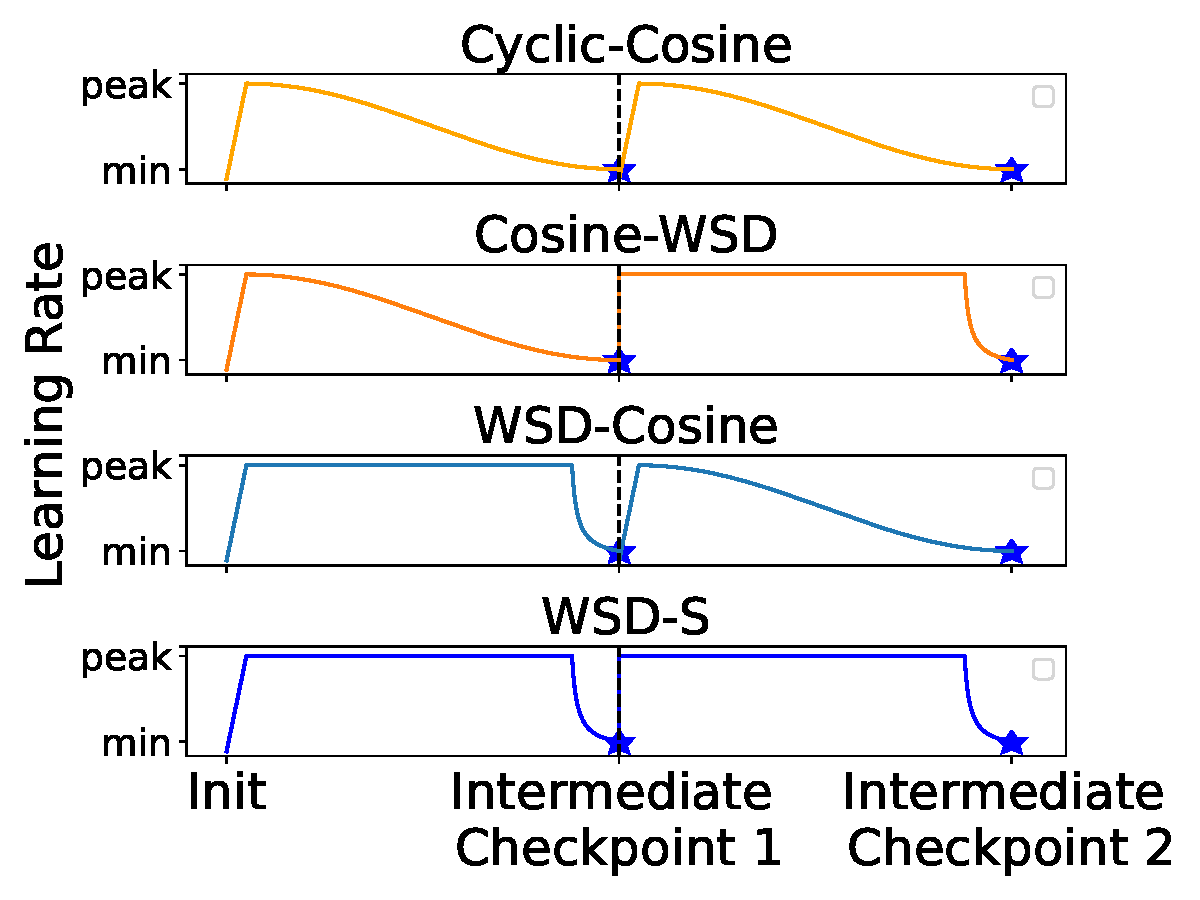
\includegraphics[width=\textwidth]{figures/arxiv/schedule_control.pdf}
    \end{subfigure}
    \begin{subfigure}[b]{0.49\textwidth}
        \centering
        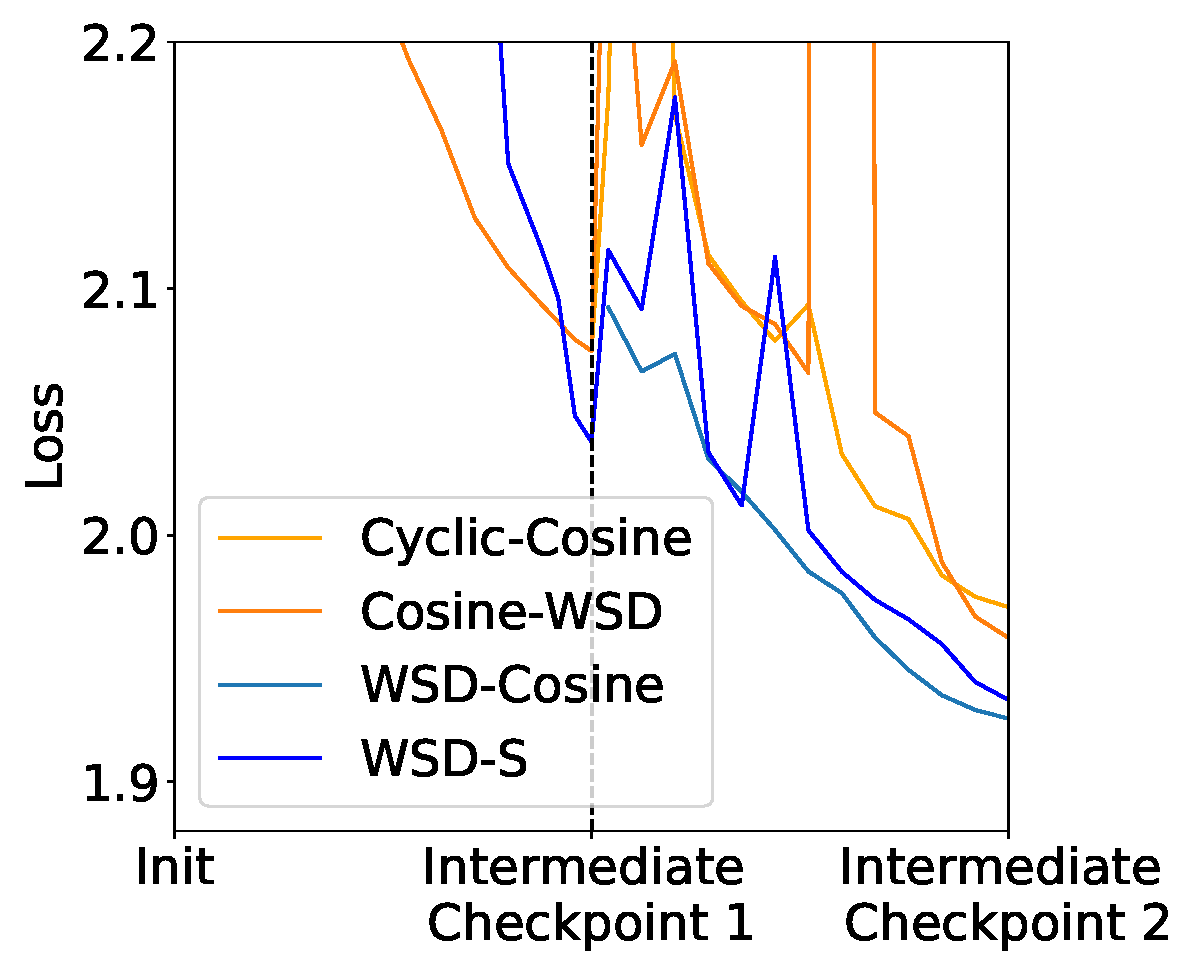
\includegraphics[width=\textwidth]{figures/arxiv/schedule_control_result.pdf}
    \end{subfigure}
    \caption{\textbf{Cosine Learning Rate Implicitly Hurts the Models for Future Continual Learning.} We show that while $\wsd$ and the cosine learning rate schedule may produce similar validation loss in a single run, a model trained with the cosine learning rate schedule is implicitly hurt compared to the model trained with $\wsd$ for future Continual learning. On the 0.6B models, after training the models for 50B tokens using both $\wsds$ and the cosine learning rate schedule, we continually train two models for another 50B tokens using both learning rates. We observe that the model trained with $\wsds$ consistently outperforms the model trained with the cosine learning rate when used as the starting point for further training.}
    \label{fig:comparison}
\end{figure}



\textbf{Implementation.} We set the batch size to 1024 and fixed the peak learning rate for the same model size for all the methods. For the 0.1B and 0.3B models, we use a peak learning rate of 6e-4, and for the 0.6B and 1.2B models, we use a peak learning rate of 4e-4. These values are chosen following current empirical practice (e.g. see \cite{groeneveld2024olmoacceleratingsciencelanguage}). We set the minimal learning rate to 0.1 of the peak learning rate. We use a TPU v3-256 model to train the model with the Levanter framework in Jax \citep{jax2018github, levanter}. The  fraction of time spent decaying is chosen to be $10\%$. The only exception is that when running $\wsd$ on the 0.3B models, we encounter a loss spike after training for 22.5B tokens and decay at the checkpoint trained for 22B tokens instead.
This change is in favor of $\wsd$ in our comparison between $\wsds$ and $\wsd$.
The detailed hyperparameters are deferred to~\Cref{app:exp}.











\subsubsection{Results}
\begin{figure}[t]
    \centering
        \begin{subfigure}[b]{0.24\textwidth}
            \centering
            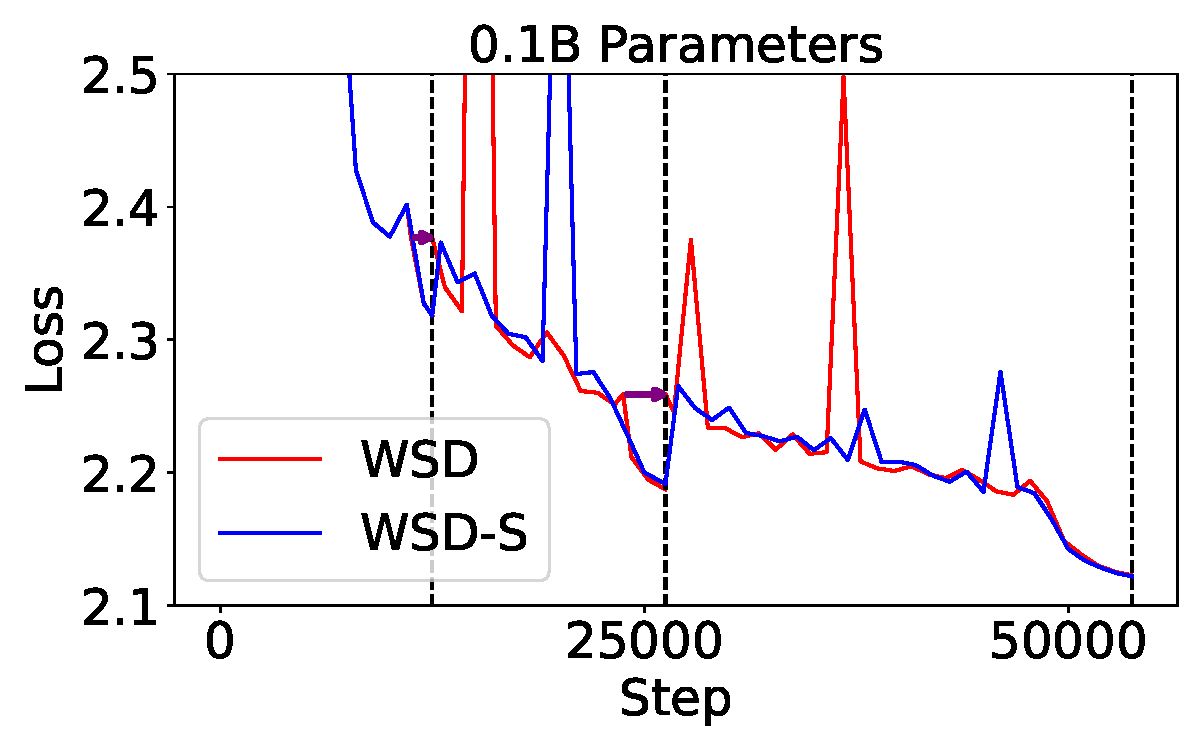
\includegraphics[width=\textwidth]{figures/arxiv/0.1B_with_wsd.pdf}
        \end{subfigure}
        \begin{subfigure}[b]{0.24\textwidth}
            \centering
            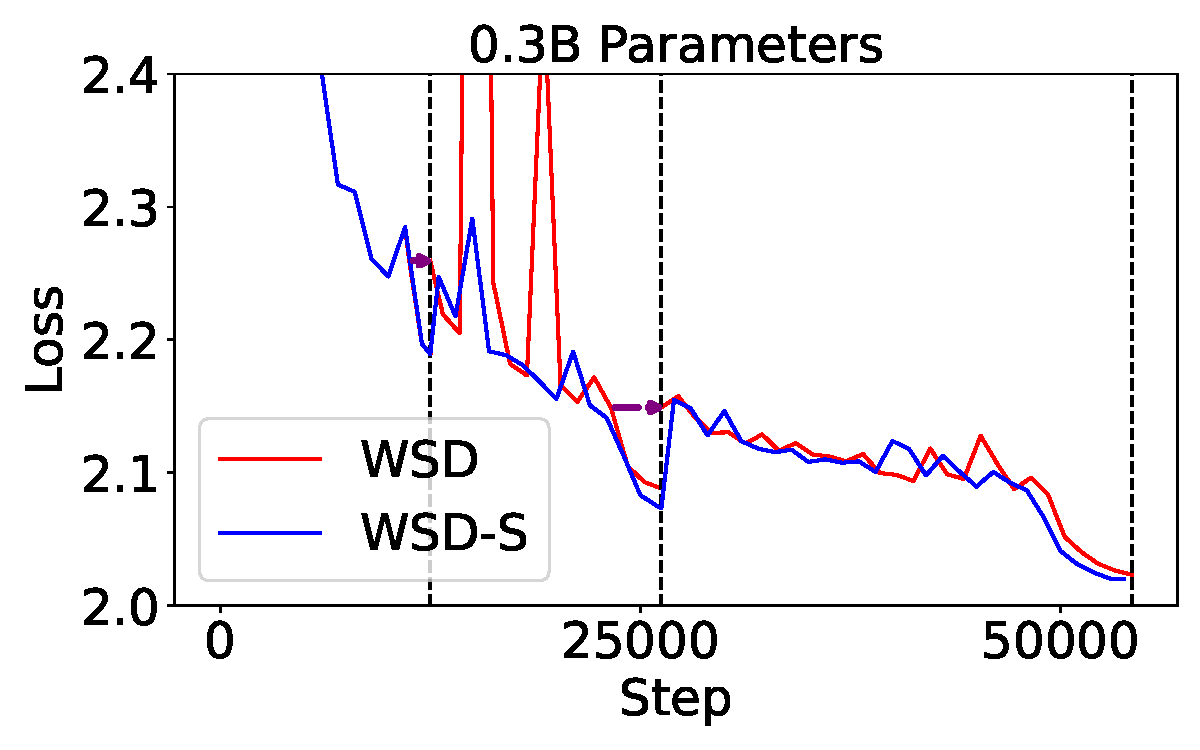
\includegraphics[width=\textwidth]{figures/arxiv/0.3B_with_wsd.pdf}
        \end{subfigure}
        \begin{subfigure}[b]{0.24\textwidth}
            \centering
            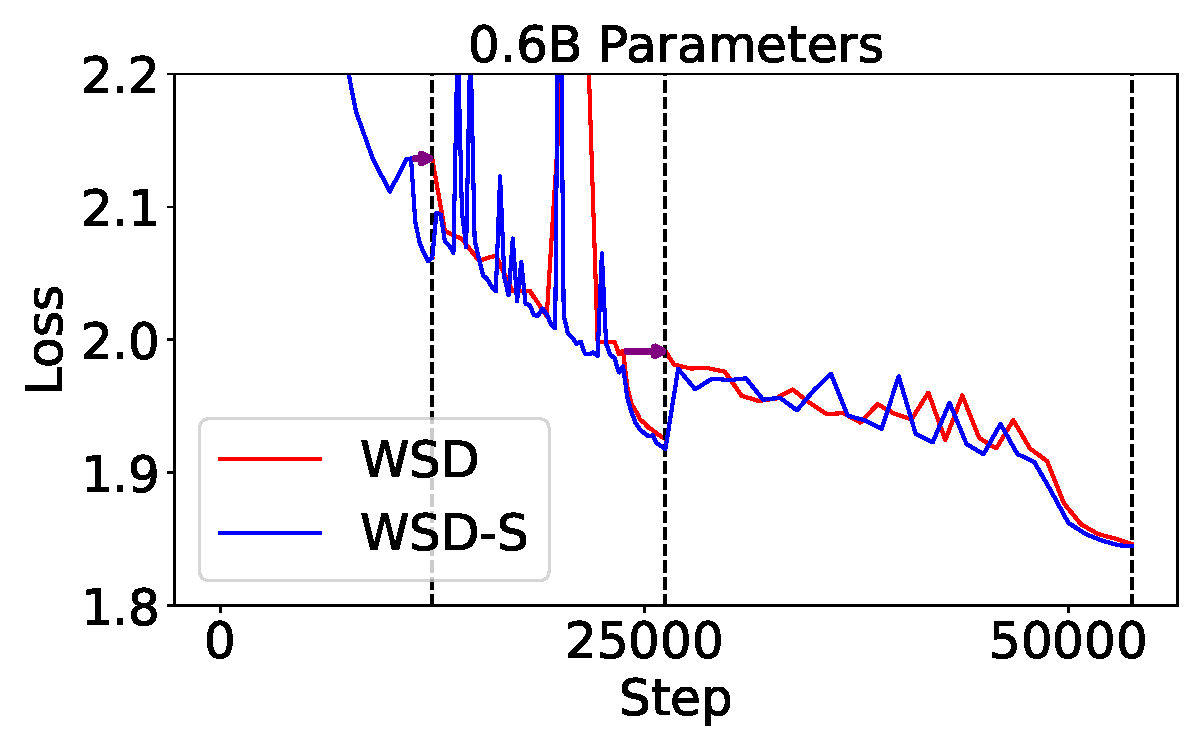
\includegraphics[width=\textwidth]{figures/arxiv/0.6B_with_wsd.pdf}
        \end{subfigure}
        \begin{subfigure}[b]{0.24\textwidth}
            \centering
            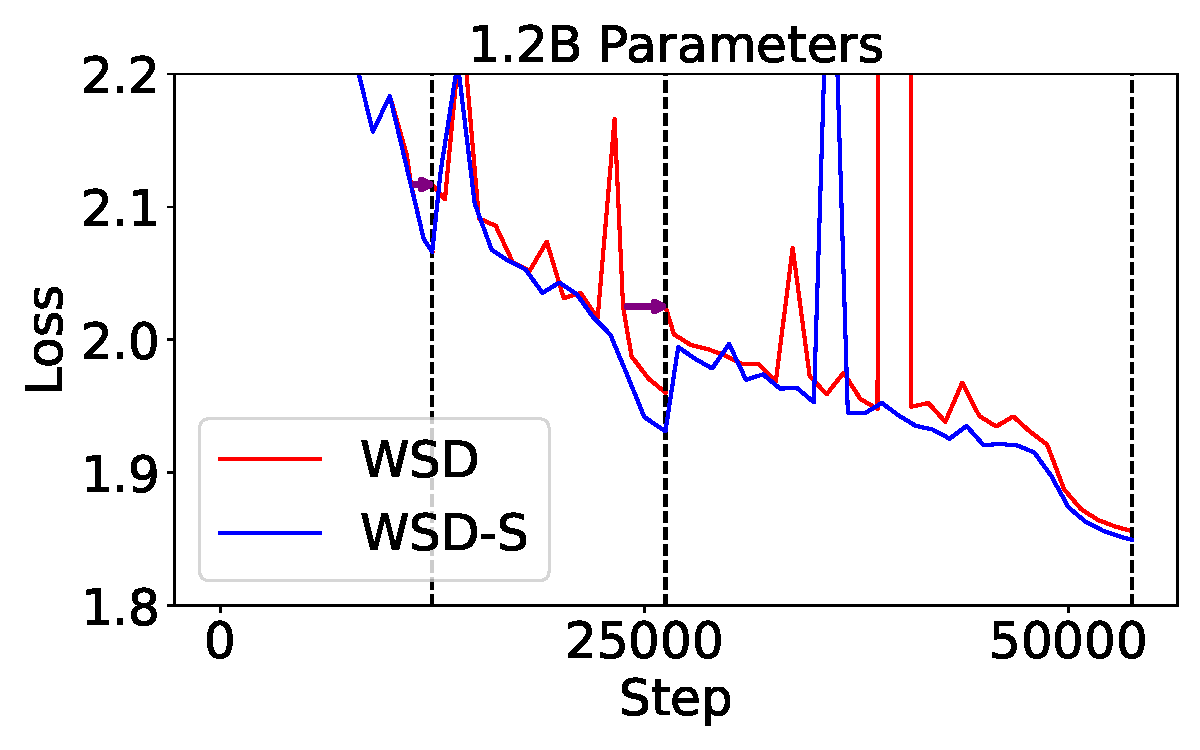
\includegraphics[width=\textwidth]{figures/arxiv/1.2B_with_wsd.pdf}
        \end{subfigure}
        \quad
    \caption{\textbf{Comparison With $\wsd$.} We show that $\wsds$ performs favorably compared with $\wsd$ when the total computes is fixed, achieving a consistent improvement over $\wsd$ on all the model sizes when trained for approximately 200B tokens.}
    \label{fig:wsd}
    \vspace{-0.2in}
\end{figure}


\textbf{$\wsds$ performs competitively with $\cosineoracle$.} The three endpoints of $\wsds$ are set at 50B, 100B, and 200B tokens for all models. As shown in \Cref{fig:main}, $\wsds$ delivers competitive results compared to $\cosineoracle$ in a single run.

\textbf{$\wsds$ significantly outperforms $\cycliccosine$.} 
We compare the $\cycliccosine$ and the $\wsds$ on 0.6B models with a total token budget of 100B tokens. Both schedules reduce to a minimal learning rate at 50B tokens to obtain an intermediate checkpoint. Our results show that $\wsds$ outperforms $\cycliccosine$ with a significant performance gap of 4e-2 (\Cref{fig:comparison}). A common belief is that loss spiking after increasing the learning rate is the main cause of the performance loss in $\cycliccosine$. However, this belief does not explain the advantage of $\wsds$. We hypothesize that a model trained with a small learning rate for too long, as with Cosine, is implicitly hurt compared to a model trained with a large learning rate for the majority of the run, as with $\wsd$ or $\wsds$. 

To show that the model trained with $\wsd$ is more suitable for continual training, we conducted ablation studies by interchanging the schedules in the latter half of the runs to create two new learning rates (Cosine-$\wsd$ and $\wsd$-Cosine). Among the four runs, the model trained using $\wsd$ for the first half consistently achieved lower loss in continual learning, indicating that $\wsd$ produces models more suitable for continual learning, even after learning rate decay.


\textbf{$\wsds$ matches (and slightly outperforms) $\wsd$ given the same total compute.} For $\wsd$, we adopt the following comparison methodology: assuming a 10$\%$ decay portion, to get three checkpoints at 12.5k, 25k, and 50k steps, $\wsd$ then requires corresponding total steps of 12.5k, 26.25k, and 53.75k.  Hence, we examine whether $\wsds$ can output three models of matching or better performance in the same corresponding steps (see \Cref{fig:wsd}). Our results suggest that $\wsds$ consistently outperforms $\wsd$ when trained on 200B tokens and underperforms $\wsd$ only on the smallest scale experiments when we trained 0.1B models for 25k steps. As this is the smallest scale experiment, we conclude that $\wsds$ has a slight advantage over $\wsd$ when the total compute is fixed. This matches our intuition that $\wsds$ can reuse the decay phases of previous checkpoints, leading to a more efficient use of the total compute. As a simpler version of $\wsd$, $\wsds$ is more user-friendly for open-source pretrained models, allowing users to continue training the final checkpoint without needing intermediate ones given that the pretrained models are trained with $\wsd$ or $\wsds$.

\begin{figure}[t]
    \centering
    \begin{subfigure}[b]{0.28\textwidth}
        \centering
        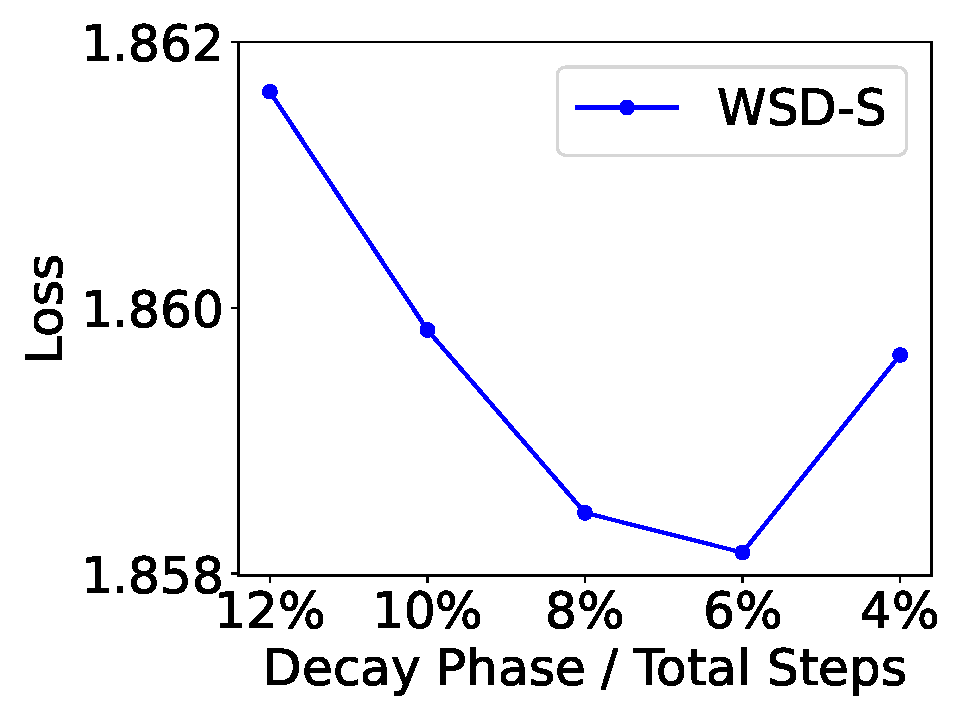
\includegraphics[height=3cm,width=\textwidth]{figures/arxiv/1.2B_ablation.pdf}
        \caption{1.2B Models on 200B tokens}
        \label{fig:1B200B}
    \end{subfigure}
    \hfill
    \begin{subfigure}[b]{0.28\textwidth}
        \centering
        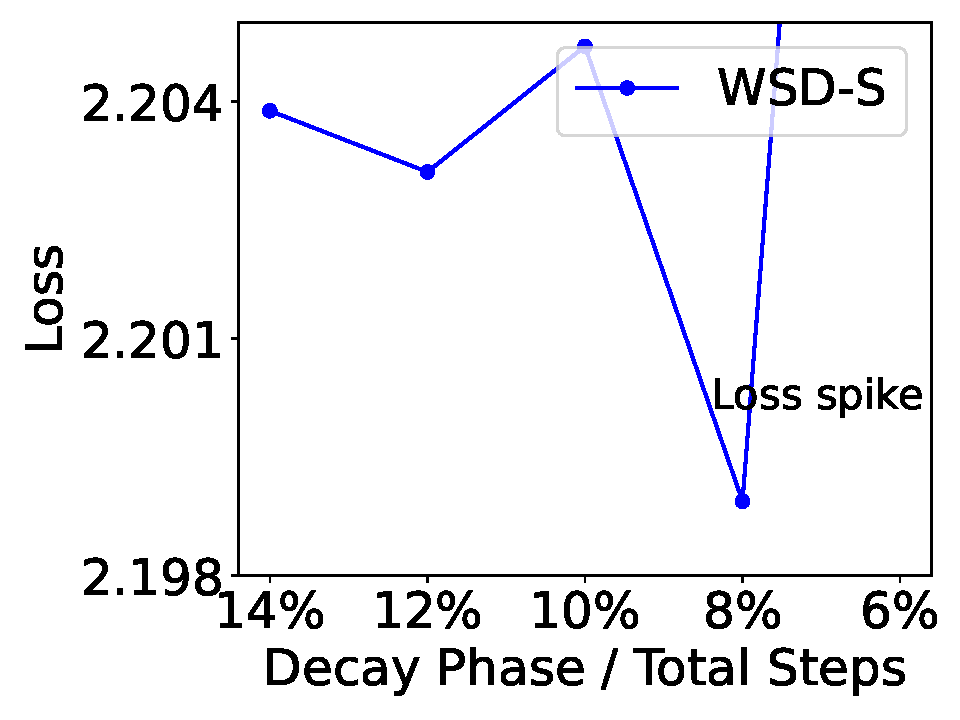
\includegraphics[height=3cm,width=\textwidth]{figures/arxiv/0.1B_ablation.pdf}
        \caption{0.1B Models on 100B tokens}
        \label{fig:100M50B}
    \end{subfigure}
    \hfill
    \begin{subfigure}[b]{0.4\textwidth}
        \centering
        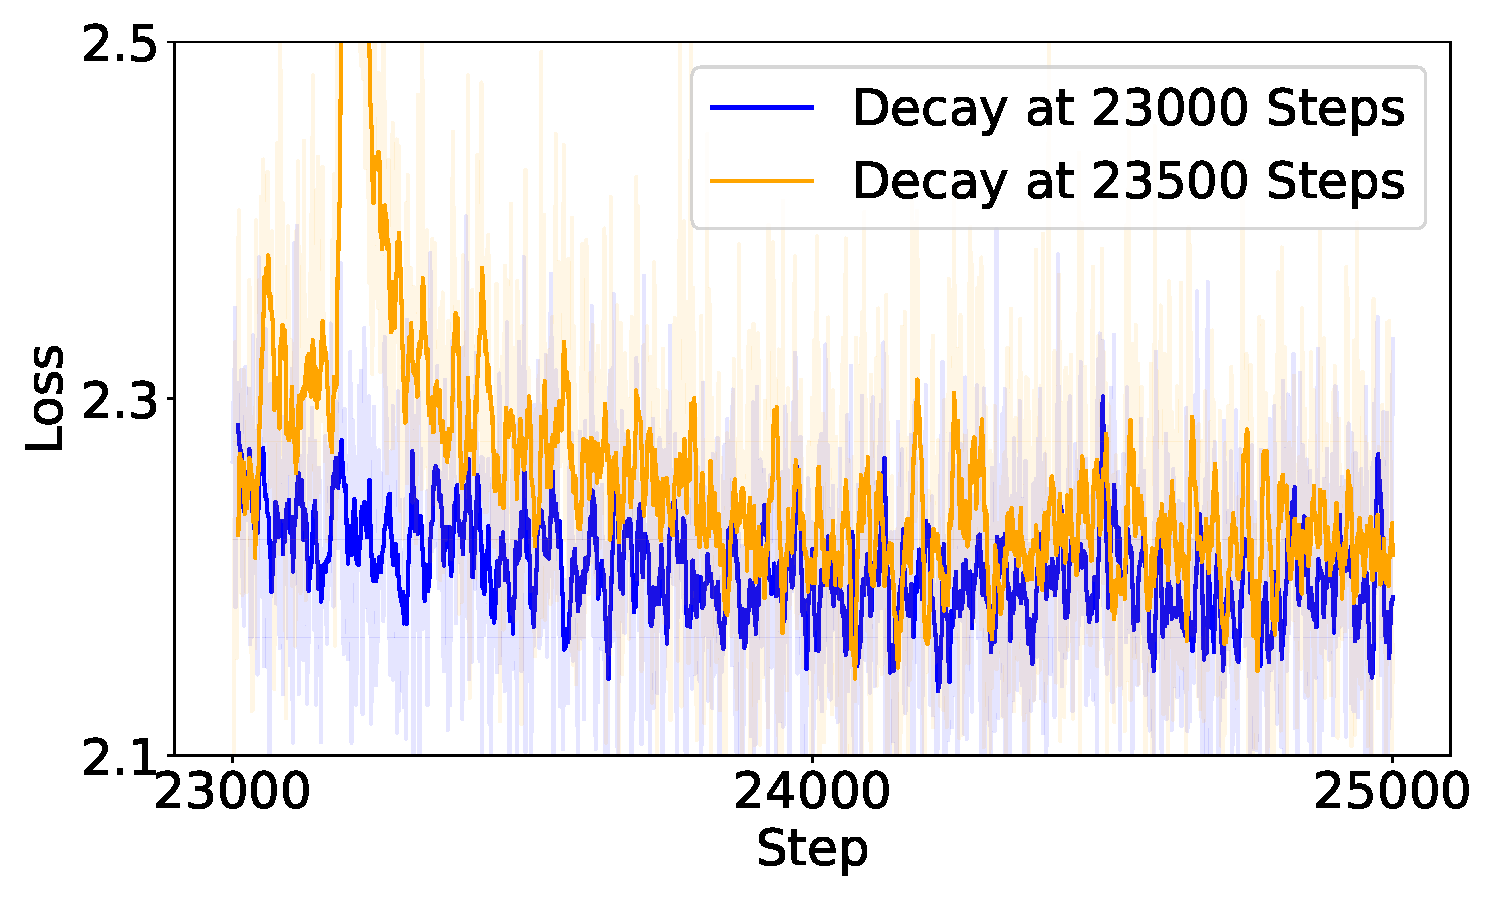
\includegraphics[height=3cm,width=\textwidth]{figures/arxiv/failure.pdf}
        \caption{0.1B Models on 100B Tokens.
         Decay Near a Loss Spike (6\%)}
        \label{fig:spikeobscure}
    \end{subfigure}
    \caption{\textbf{Ablation Study on the Sensitivity of Fraction of Time Decaying}. This study examines two settings: a smaller scale with 0.1B parameters trained on 100B tokens (middle figure) and a larger scale with 0.6B parameters trained on 200B tokens (left figure). The results indicate that the final performance is similar when the decay phase is 8\%-12\% of the total training steps. However, the right figure demonstrates a significant performance loss when decaying near a loss spike. It compares two training loss curves with decay phases of 8\% and 6\% of the total compute on the 0.lB models, where the latter starts immediately after a loss spike, leading to a validation loss increase of 2e-2.}
    \label{fig:portion}
    \vspace{-0.2in}
\end{figure}

\textbf{$\wsd$ and $\wsds$ is not sensitive to the fraction of time spent decaying} We conclude with an ablation study on the fraction of time spent decaying, and the result is shown in~\Cref{fig:portion}.
The final performance matches tightly within the range of $8\%$ to $12\%$, showing small sensitivity to the choice of the decay portion. 

However, in our experiments, we observe that decaying near a loss spike can lead to a significant performance loss (\Cref{fig:portion}, right).With the large learning rate, the training runs tend to be very volatile and there are multiple loss spikes in the training (see~\Cref{fig:main}). If a decay happens closely \emph{after} a loss spike and the loss has not yet decreased to its original level, it is typical that the final validation loss will be worse by 1e-2 or even more. We observe the same phenomenon for $\wsd$, and when such a scenario happens, we suggest either running longer till the loss stabilizes or rolling back to a slightly earlier checkpoint before the loss spikes and decays from there.







